\chapter{Background}\label{gen:sec:background}
\markboth{Background}{Background}

In this chapter, I provide background on graph processing including descriptions of the algorithms and input graphs used for evaluation in this thesis.
I then describe the \graphit DSL which allows programmers to describe graph algorithms separate from their scheduling optimizations.
Finally, I provide background on manycore architectures and describe the representative manycore that we target with our code generator. 
%\todo{write background on graph processing, graph topologies, graphs used in this thesis, and algorithms used}

%\section{The Graph Abstraction}\label{thesis:background:graphproc}
\todo{talk about graph processing at a high level, talk about related data, maybe storage format?}
\section{Graph Topology}\label{thesis:background:topology}
\todo{planar vs. scale-free, properties of each}
A scale-free or social network graph has a degree distribution that follows a power-law, at least asymptotically~\cite{barabasi1999emergence}.

\section{Graphs used in this Thesis}\label{thesis:background:graphs}
In this work, we use a diverse set of graphs for evaluation.
These graphs and their properties are listed in Table~\ref{tab:graphprop}.
A graph's topology greatly impacts a workload's characteristics and performance, so it is important to perform evaluation on a diverse set of graphs~\cite{beamer2015locality}.
We use a mix of real-world and synthetic graphs in our evaluation and primarily focus on social network topologies. 

The real-world graphs we use come from a variety of sources. 
We examine two real-world social network graphs: Pokec and LiveJournal which represent the links between users in their online communities. 
We also consider the Hollywood graph which considers professional relationships.
It links together actors that have performed together.
These are all representative of a scale free or social network topology as they all have a low effective diameter and power-law degree distribution.
In contrast, we also use three road network graphs in our evaluations. 
These are mesh topologies with low average degree and high diameter. 

In addition to these real-world graphs, we fill out our set of graphs with three synthetic graphs.
Like in the Graph500 benchmark, we generate several kron graphs of varying size using the \kron generator~\cite{murphy2010graph500}.
These graphs model a social network and follow a power-law degree distribution. 


\begin{table*}[h]
\centering
\begin{tabular}{lllll}
\toprule
\textbf{Name} & \textbf{Description} & \textbf{Vertices} & \textbf{Edges} & \textbf{Degree} \\ \midrule
Kron18 & \kron generated~\cite{leskovec2005realistic,leskovec2010kronecker} & 262,144 & 4,194,304 & 16 \\
Kron20 & \kron generated~\cite{leskovec2005realistic,leskovec2010kronecker} & 1,048,576 & 16,777,216 & 16 \\
Kron22 & \kron generated~\cite{leskovec2005realistic,leskovec2010kronecker} & 4,194,304 & 67,108,864 & 16 \\
Pokec & social network~\cite{snapnets} & 1,632,803 & 30,622,564 & 18.8 \\
LiveJournal & social network~\cite{mislove2007measurement,davis2011university} & 4,847,571 & 85,702,474 & 17.6 \\
Hollywood & movie collaborations~\cite{boldi2011layered,boldi2004webgraph,davis2011university} & 1,139,905 & 112,751,422 & 98.9\\
RoadCA & CA road network~\cite{davis2011university} & 1,971,281 & 5,533,214 & 2.8\\
RoadCentral & Central road network~\cite{davis2011university} & 14,081,816 & 33,866,826 & 2.4\\
RoadUSA & USA road network~\cite{road-graph} & 23,947,347 & 57,708,624 & 2.4\\
\bottomrule
\end{tabular}
\caption{List of graphs used in this thesis and their properties.All of the graphs come from real-world data except
the three \kron graphs. Throughout our evaluation, we list the subsets of these graphs that are being evaluated.}
\label{tab:graphprop}
\end{table*}

\section{Algorithms used in this Thesis}\label{thesis:background:algorithms}
%\todo{explain bfs, sssp (delta + bellmanford), pr, cc, bc, etc. in detail}
In this thesis we explore a variety of graph processing algorithms. 
We select them based on their popularity in graph-processing evaluations~\cite{beamer2016thesis} and for the different behaviors that they exhibit.
The algorithms we examine can be classified as traversal-centric or compute-centric algorithms. 
Traversal-centric or frontier-based algorithms start from a given source vertex and perform computation on vertices by traversing outwards from the source vertex.
Compute-centric algorithms operate on the entire graph in parallel and tend to iteratively apply updates until the algorithm converges.

\paragraph{Breadth First Search (BFS)}\mbox{}\\
BFS is a building block of many graph algorithms. 
It is not an algorithm but really a graph traversal order. 
BFS visits every vertex at a given depth of the graph before moving on to the next depth level.
We turn it into an algorithm by discovering and tracking the parent vertex ID of each vertex reachable from a given source vertex.

\paragraph{Single Source Shortest Path (SSSP)}\mbox{}\\
SSSP is an algorithm that builds off of BFS to compute the distances of the shortest paths from a given source vertex to every other reachable vertex in the graph.
This is usually performed on a weighted graph, so the weights of edges are used in calculating the distance of a path.
We only consider graphs with non-negative edge weights in this work.
We examine two different SSSP algorithms, frontier-based Bellman-Ford and Delta-stepping.

Frontier-based Bellman-Ford trades off repeated accesses to edges for increased parallelism. 
It uses relaxation where approximations of the distances to each vertex are replaced by shorter distances until the algorithm converges on the correct solution.
Unlike Dijkstra's, the classical SSSP algorithm, there is no notion of priority in Bellman-Ford and all edges active in the frontier are relaxed in every iteration.

The delta-stepping algorithm~\cite{meyer2003delta} increases parallelism by using a notion of relaxed priority. 
Delta-stepping coarsely sorts the vertices of the graph by distance into buckets of width $\Delta$.
This allows for all vertices in a bucket to be processed in parallel. 
Like Bellman-Ford, this does result in some vertices being processed multiple times, but the frequency with which this occurs can be reduced by reducing the value of $\Delta$.
If $\Delta=1$, the algorithm effectively becomes Dijkstra's, and if $\Delta=\inf$, the algorithm behaves like Bellman-Ford. 

\paragraph{PageRank (PR)}\mbox{}\\
PR calculates the importance or "popularity" of each vertex in a graph and was originally developed to sort web search results~\cite{page1999pagerank}.
It calculates the popularity of a vertex $v$ by considering both the number of vertices that point to $v$ and the importance of those vertices that point to $v$.
PR iteratively updates the PageRank score for each vertex in the graph until the scores converge within some specified tolerance.
There has been considerable work on optimizing PageRank and finding ways to improve the convergence rate~\cite{low2010graphlab,shun2013ligra,kohlschutter2006efficient}

\paragraph{Connected Components (CC)}\mbox{}\\
The Connected Components algorithm labels all of the components in a graph. 
A connected component is a subgraph in which all vertices are connected to each other.
If an edge exists between two vertices, they are connected. 
In a directed graph, connections between vertices can be asymmetric.
This means that components of a directed graph can be strongly or weakly connected. 
In this thesis, we only consider undirected graphs and do not need to consider asymmetry of connections.
The CC algorithm labels vertices so that all vertices in the same component have the same label.

\paragraph{Betweenness Centrality (BC)}\mbox{}\\
BC is another algorithm that attempts to measure the importance of the vertices in a graph. 
It calculates a score for each vertex that measures the fraction of shortest paths that pass through the vertex.
This can be computationally expensive as the algorithm needs to compute the shortest paths for all pairs of vertices in the graph.
This is often done by computing the All Pairs Shortest Path algorithm which executes SSSP for every vertex in the graph as a source vertex. 
Calculating all of the shortest paths can be both compute and memory intensive. 
The Brandes algorithm reduces the memory requirements by compacting the critical information from a SSSP execution into a single variable~\cite{brandes2001faster}.
We also compute BC on an unweighted graph in this work, which allows us to use BFS traversals to compute the shortest paths. 


\newcommand{\graphformatfig}{
\begin{figure}[h]
    \centering
    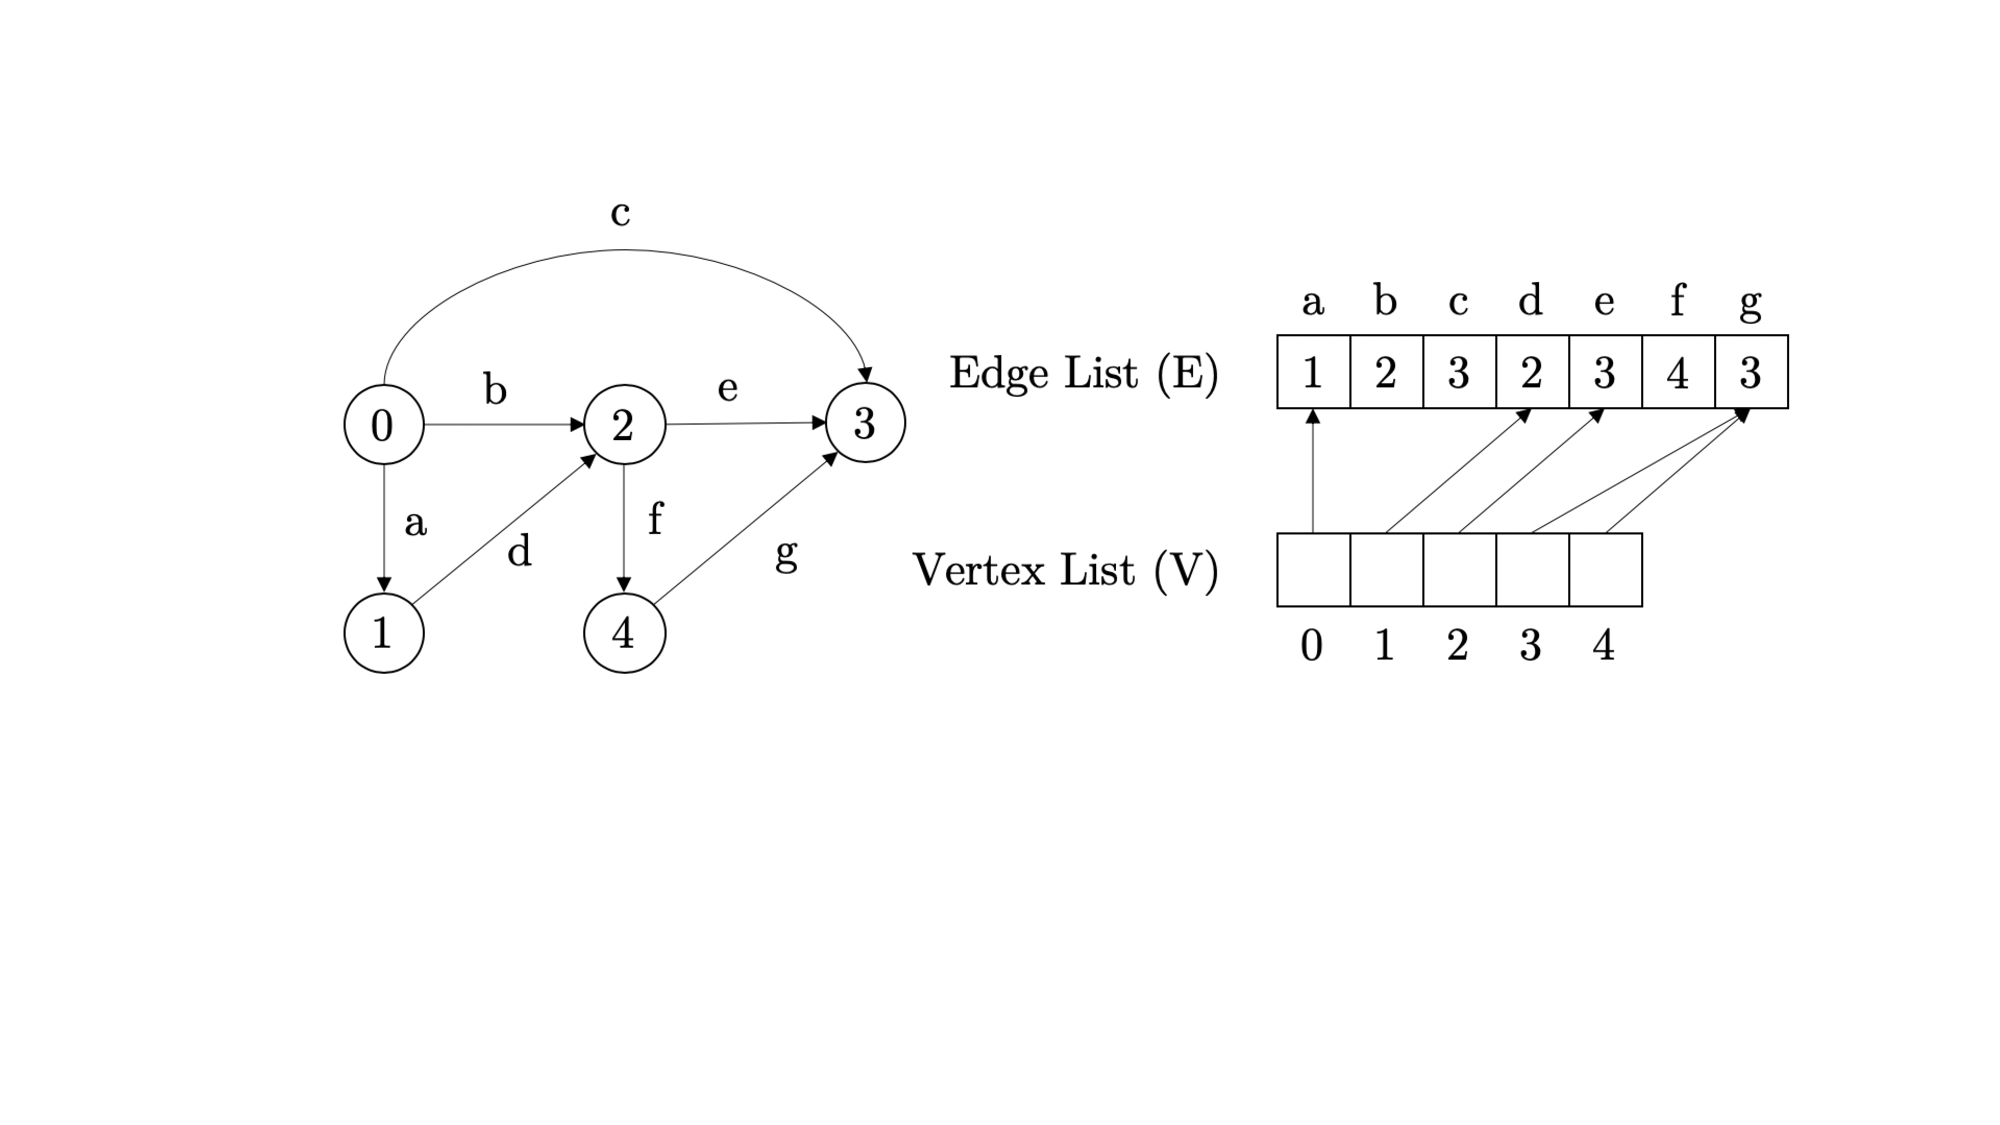
\includegraphics[width=0.8\textwidth]{graphit-figures/graph-format-figure.pdf}
    \caption{The CSR graph format that we use to store graph data on the manycore. For weighted graphs, the weight is stored with each element in the edge array.}
    \label{pap:generals2020:sec:background:fig:graphformat}
\end{figure}
}
\section{GraphIt: A Graph Processing Domain-Specific Language}\label{pap:generals2020:sec:graphit}

GraphIt is a domain-specific language for graph processing applications~\citep{zhang2018graphit}.
Like Halide~\citep{ragan2013halide}, GraphIt separates the description of the algorithm from the scheduling of the computation. A separate algorithm language and scheduling language are used to specify graph programs in GraphIt. This separation of description and schedule allows users to express computation more flexibly.
Listing~\ref{pap:generals2020:sec:background:lst:graphit} shows an example GraphIt program implementing Breadth-First Search (BFS).

\begin{lstlisting}[language=graphit, 
                   caption=GraphIt code for Breadth-First Search (BFS),
                   label=pap:generals2020:sec:background:lst:graphit]
const edges : edgeset{Edge}(Vertex,Vertex);
var frontier : vertexset{Vertex} = new vertexset{Vertex}(0);
const parent : vector{Vertex}(int) = -1;

func updateEdge(src : Vertex, dst : Vertex)
    parent[dst] = src;
end

func toFilter(v : Vertex) -> output : bool
    output =  parent[v] == -1;
end

func main()
    // frontier setup
    while (frontier.getVertexSetSize() != 0)
      #s1# frontier = edges.from(frontier).to(toFilter).applyModified(updateEdge,parent,true);
    end
end

schedule:
  program->configApplyDirection("s1", "DensePull")->generateManycoreCode();
\end{lstlisting}

\subsection{Graph Representation}
Graphs are represented by \lstinline[language=graphit]{edgeset} and \lstinline[language=graphit]{vertexset} structures.
The edges between nodes are stored as an \lstinline[language=graphit]{edgeset}, and any vertex specific data is stored as a \lstinline[language=graphit]{vertexset}.
Line~1 and Line~2 of Listing~\ref{pap:generals2020:sec:background:lst:graphit} demonstrate the declaration of the \lstinline[language=graphit]{edgeset} variable \lstinline[language=graphit]{edges} and  \lstinline[language=graphit]{vertexset} variable \lstinline[language=graphit]{frontier}. 
Any data associated with elements in an \lstinline[language=graphit]{edgeset} or \lstinline[language=graphit]{vertexset} is stored as a \lstinline[language=graphit]{vector}.
Line~3 of Listing~\ref{pap:generals2020:sec:background:lst:graphit} shows the declaration of a \lstinline[language=graphit]{vector} variable, \lstinline[language=graphit]{parent}, that contains data associated with the vertices in the graph.

GraphIt uses Compressed Sparse Row (CSR) graph format for these data structures, illustrated in Figure~\ref{pap:generals2020:sec:background:fig:graphformat}.
CSR format represents a graph with two arrays: a vertex list and an edge list.
The edge list contains the destination vertex for each edge in the graph and contains $|E|$ elements where $E$ is the set of edges in the graph.
In the case of a weighted graph, the edge list is stored as an array of tuples, with each element in the array containing the destination vertex id and the weight of the edge.
The vertex list contains $|V|$ elements where $V$ is the set of vertices in the graph. 
Each element in the vertex list is an index into the edge list array.
This index corresponds to the start of the edges for which that vertex is the source vertex.
The number of edges for a vertex $v$, or its degree, is $vertex\_list[v+1] - vertex\_list[v]$.
The generated code operates on these arrays to perform computation.

\graphformatfig


\subsection{Algorithm Representation}
An algorithm in GraphIt is written as operations on \lstinline[language=graphit]{edgeset} and \lstinline[language=graphit]{vertexset} datatypes. 
Graphit provides several operators that perform computation on these types, but the most common are the \lstinline[language=graphit]{filter} operator and \lstinline[language=graphit]{apply} operator.
The \lstinline[language=graphit]{filter} operator takes a function and a set, applies the function to each element in the set, and returns a set of elements where the function returned true.
The \lstinline[language=graphit]{apply} operator takes a function and set as input and applies the function to each element in the set. %, and returns the resulting set of modified elements.
GraphIt also provides other built-in operators like \lstinline[language=graphit]{applyModified}, that takes a function and a set, applies the function to each element in the set, and returns a vertexset that contains vertices that were updated by the input function. 
This operator is used to construct frontiers in iterative graph algorithms. 
Listing~\ref{pap:generals2020:sec:background:lst:graphit} demonstrates how these operators can be used to write BFS.

Line~16 of Listing~\ref{pap:generals2020:sec:background:lst:graphit} demonstrates two uses of the \lstinline[language=graphit]{filter} operator and one use of the \lstinline[language=graphit]{applyModified} operator. 
The first filter application (\lstinline[language=graphit]{from(frontier)}) selects only edges with source vertices that are in the current frontier. 
The second filter application (\lstinline[language=graphit]{to(toFilter)}) uses the \lstinline[language=graphit]{toFilter} function, defined on line~9, to select edges with destination vertices that haven't been previously visited.
Next, an \lstinline[language=graphit]{applyModified} operator is applied to this filtered set of edges.
This operator computes the edge traversal of BFS and returns a vertexset containing the vertices that were updated by the \lstinline[language=graphit]{updateEdge} function defined on line~5.
This \lstinline[language=graphit]{vertexset} becomes the new frontier for the next iteration of the while-loop.
%\todo[inline]{Check all line-number references}

\subsection{Schedule Representation}
GraphIt provides a wide range of scheduling options, i.e., by specifying traversal direction, by specifying the level of parallelism, or by using load balancing techniques for parallel operators.
Labels are used to indicate which operators in the algorithm description the scheduling optimizations should be applied to.
The separation of the algorithm description and schedule allows developers to iterate through different scheduling optimizations and is a key part of GraphIt.
The schedule finishes by generating code for the target device.
The schedule description always follows the algorithm description in GraphIt.

The schedule for BFSs starts with the \lstinline[language=graphit]{schedule} declaration on Line~20 of Listing~\ref{pap:generals2020:sec:background:lst:graphit}. Line~21 specifies that the schedule for label \lstinline[language=graphit]{#s1#} should be "Dense Pull". This schedule is described in Section~\ref{sec:method}
Finally, the schedule specifies that the code generator should generate code for the target device. 

\subsection{Code Generation}
GraphIt's code generator takes an algorithm and schedule and generates device-specific code.
Graphit first parses the algorithm and schedule using the frontend to produce the Intermediate Representation. 
Next, the compiler performs dependency analysis and enforces restrictions on read-write accesses and reduction operators. 
Once the compiler verifies the validity of the algorithm and schedule, the backend generates code for the target device and host (if necessary).
%Section~\ref{sec:method} describes how our back end generates manycore code.


\newcommand{\manycoreArchFigure}{
\begin{figure}[t]
    \centering
    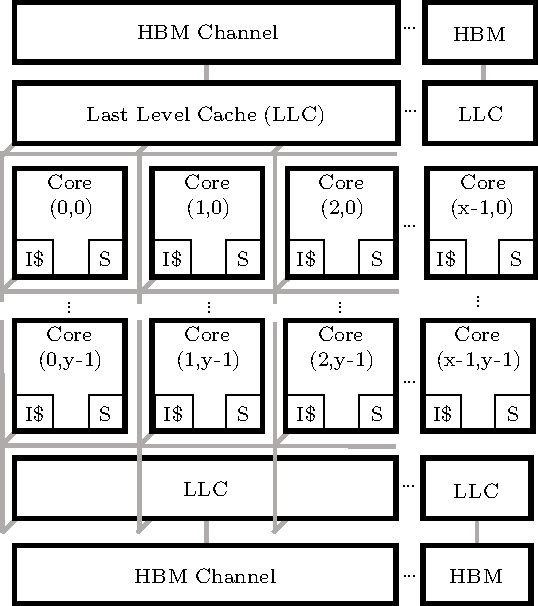
\includegraphics[scale=0.8]{graphit-figures/manycore-arch.pdf}
    \caption{Block diagram of the general manycore architecture targeted in
      this thesis. A 2D-Mesh Network-on-Chip connects general-purpose
      computation cores and Last Level Caches (LLC). Each LLC connects to a single
      independent High-Bandwidth Memory (HBM) channel.}
    \label{pap:generals:sec:architecture:fig:hbarch}
\end{figure}
}
\section{Manycore Architectures} \label{pap:generals:sec:architecture}
Manycore architectures provide thread-level parallelism and flexibility with hundreds to thousands of general-purpose cores~\cite{ramey2011tilera, davidson2018celerity, gwennap2011adapteva, agathos2015parallela, taylor2004raw}.
Cores are arranged in two-dimensional arrays and interconnected with mesh-style networks for communication.
This network of cores is surrounded by multiple channels of memory to provide sufficient bandwidth and parallelism to sustain computation.
Cores within the architecture communicate explicitly through memory~\cite{davidson2018celerity} or message passing \cite{gwennap2011adapteva}, implicitly through coherence protocols~\cite{ramey2011tilera}, or both using inter-core result networks \cite{taylor2004raw}.
Communication allows cores to cooperate and solve large parallel tasks.
The quantity of cores and diverse communication patterns means that manycore architectures provide a flexible parallel computation fabric that can be tailored to fit application requirements or the structure of graph input data \cite{lumsdaine2007challenges}.

In this section, I describe a representative manycore architecture that we use to evaluate our code generator.
The cores are tiny, performance-optimized scalar cores that implement a RISC-V instruction set.
Each core has a software-managed scratchpad memory for low-latency storage and inter-thread communication.
Data cache lines do not move between cores, eliminating coherence overhead and false sharing.
The memory system is designed to expose memory parallelism and bandwidth to service memory requests from hundreds of concurrent threads.
This architecture is emblematic of Single Program Multiple Data (SPMD) parallel machines where collections of cores are loaded with the same program, but each core computes on different input data.

This section provides a overview of the target manycore
architecture depicted in
Figure~\ref{pap:generals:sec:architecture:fig:hbarch}. The
architecture is composed of efficient general-purpose processor cores,
Last Level Caches (LLCs), a 2D-Mesh Network on Chip, and High-Bandwidth
Memory (HBM) channels.
%% Fluff -M
%The system is designed for efficient
%computation of general-purpose scientific, graph, and machine-learning
%workloads that can exploit the unprecedented memory-level parallelism
%provided by the independent cores, caches, and HBM channels.

\manycoreArchFigure

\subsection{Network-On-Chip}
Communication is provided by a 2D-Mesh Network-on-Chip (NoC) that
interconnects Last Level Caches and general-purpose cores. The
NoC supports point-to-point communication between endpoints using
shared memory. All addressable endpoints within the network are
assigned a unique global address range. This provides a PGAS-like
(Partitioned Global Address Space) memory model for execution.

\subsection{Memory System}
The manycore's memory system is designed to provide the high-bandwidth memory-level parallelism required by manycore
architectures. The memory system has four hierarchy levels:
High-Bandwidth Memory (HBM), Last Level Cache (LLC), core-remote
scratchpad (S), and core-local scratchpad (S). Each level is designed
to exploit memory parallelism and exposes a trade-off between latency,
capacity, as shown in
Figure~\ref{pap:generals:sec:architecture:fig:hbarch}.

Manycore architectures require many high-bandwidth and independent
memory channels to supply data for computation, so we use
second-generation High Bandwidth Memory (HBM, or HBM2). HBM provides
two sources of memory-level parallelism: First, HBM provides
channel-level parallelism with 8 independent physical channel
interfaces per chiplet. Each channel has a maximum data transfer rate of 32
GB/s. Second, HBM provides bank-level parallelism through pipelining
commands. Commands for opening/closing banks and reading data are
overlapped to hide the latency of long-running commands. Compared to
traditional SDRAM/DIMM-based devices, HBM provides more bandwidth
per-package and parallelism and is ideal for manycore
architectures, but performance depends on exploiting channel-level and
bank-level parallelism.

The banked Last Level Caches (LLC) shown in 
Figure~\ref{pap:generals:sec:architecture:fig:hbarch} are designed
to exploit bank-level parallelism within a channel. The LLCs are located at the top and bottom of the network to reduce memory access latency.
Each bank of the LLCs is connected
to a column and is mapped to a unique address range in the NoC, and
each port maps to an exclusive set of HBM banks within the LLC's
channel to avoid concurrency and conflicts. Linear traversals through
the memory space of a LLC expose bank-level parallelism to software.

% citation: https://user.eng.umd.edu/~blj/papers/memsys2018-dramsim.pdf
%Previous work has shown that for memory intensive workloads high memory bandwidth is often not enough to achieve good performance - it is also important that the memory system expose sufficient  memory level parallelism that software can exploit \cite{li2018ppmodernhighspeeddram}. 
%We use second-generation High Bandwidth Memory (HBM2) as our system's main memory. 
%HBM is a family of SDRAM technology that has recently gained prominence in parallel architectures such as GPGPUs and Google's TPU\todo{cite}. 
%HBM2 exposes two sources of memory-level parallelism. 
%First, HBM2's interface is composed of 8, independent memory channels each with wide interfaces. 
% An HBM2 channel can support up to 30 gigabytes per second of memory bandwidth. 
%Channels can receive memory requests and transfer data in parallel.
%The second way in which HBM provides MLP is in the number of DRAM banks.
%Within a bank only one memory page can be read at a time.
%Page conflicts arise when accessing data from two different pages located in the same bank. 
%When this occurs the currently opened page needs to closed, and the new page needs to be opened.
%Crucially, the operations for opening and closing pages in different banks can be overlapped. 
%Banks are thus another important source of parallelism in DRAM. 
%More banks means more open pages at a time, which reduces page conflicts when accessing DRAM and provides more opportunities to hide paging latency.
% An HBM2 chip has 16 DRAM banks per channel or 128 banks in total for the full 8 channel system.

%Our Last-Level Caches (LLC) are non-blocking with 128 byte blocks which is similar to the LLCs found in GPUs.
%We use one LLC for each HBM channel and are shown in Figure \ref{pap:generals:sec:architecture:fig:hbarch} at the top and bottom of the NoC.

%We design our cache system to exploit the MLP provided by HBM.
%The Last-Level Cache (LLC) is implemented using an array of power and area optimized blocking subcaches. 
%These subcaches operate independently and can handle  misses in parallel. 
%Each subcache services a physical address region that maps to a unique HBM bank. 
%An important consequence of this address mapping is that page conflicts can only occur from memory requests originating from the same blocking subcache.
%This maintains the memory system's ability to exploit bank level parallelism.
%It follows from our one-to-one assignment of subcaches to DRAM banks that each HBM channel handles memory requests from 16 blocking subcaches.
%The last-level cache uses 128 byte blocks, a configuration that we have found to be optimal for maximizing DRAM bandwidth and is\todo{cite} similar to what is found in GPGPU  architectures.
%The subcaches connect to the on-chip network at the top and bottom of each column in the mesh and sit between the compute cores and main system memory as shown in Figure \ref{pap:generals:sec:architecture:fig:hbarch}.


\subsection{Computational Cores}
The computational cores in
the manycore are
throughput-optimized, general purpose processors that communicate  over the NoC.
Each core is a modified Harvard architecture with an
instruction cache (I\$), and a small program-controlled data scratchpad
(S). Local scratchpad, remote scratchpads of other tiles, and main
memory are mapped to contiguous segments in the memory
space of each core. This allows nearby cores to communicate
using shared memory with extremely low overhead. 

Each core can issue a series of non-blocking, pipelined loads and stores to the NoC until a register hazard occurs. Multiple loads in flight exploit
instruction-based memory parallelism and hide the access latency of a
single access traversing the network (Table,
Figure~\ref{pap:generals:sec:architecture:fig:hbarch}). Operations
to sequential ports exploit bank-level memory parallelism, and
operations to unique caches exploit channel-level memory
parallelism. 
%The challenge for manycore architectures, and a major contribution of this paper, is to generate code that exploits the right types of parallelism to maximize performance for an application.
Manycore architectures with HBM are challenging to generate code for because of the interplay between bank and channel-level memory parallelism required to maximize performance for an application.

%Each core can issue many pipe-lined memory commands to the 
%NoC until the register file is exhausted, or a hazard occurs.
%Multiple loads in flight exploit instruction-level memory parallelism and
%hide the access latency of a single access traversing the network 
%(Table, Figure~\ref{pap:generals:sec:architecture:fig:hbarch}). 
%Loads to different memory banks exploit cache-level parallelism, and bank-level parallelism in the HBM. 
%Loads to different channels exploits channel-level memory parallelism. 
%The challenge for manycore architectures, and major contribution of this paper, is to generate code that 
%exploits the right types of parallelism to maximize performance for an application.

\subsection{Execution Model}
The manycore architecture operates under a Single Program Multiple
Data (SPMD) execution model where each core executes the same program
independently from all other cores. Multiple cores are aggregated into
rectangular \textit{groups} to perform computations that may require
cooperation. Cores in a group communicate through shared memory and
synchronize using dedicated barrier primitives. Groups can be executed
in parallel if resources are available, or sequentially if not. Ordering
between groups is not guaranteed. This programming abstraction can 
exploit the memory parallelism available in manycore architectures.

The manycore architecture described here is connected to a host	CPU, and
program execution is managed by a driver. Host programs	allocate
regions within the memory system and copy data from the host to the device,
launch parallel or sequential groups, and copy data back to the	host.
This process continues until all groups have launched and finished
execution. Once completed, the result can be copied back from the device
to host.

\section{Chapter Summary}
In this chapter, I first described graph processing at a high level before describing the behavior and structure of algorithms and input graphs used for evaluation in this thesis.
I then described the \graphit DSL and its benefits.
In chapter~\ref{gen:sec:graphitbackend} we use \graphit to implement our code generation framework as a backend to the language.
I also provided a description of the manycore architecture that we target in this thesis.